\documentclass{article}
\usepackage[utf8]{inputenc}
\usepackage[colorinlistoftodos]{todonotes}
\usepackage{setspace}
\usepackage[margin = 1in]{geometry}
\usepackage{amsmath}
\usepackage[
    backend=biber,
    style=authoryear,
    natbib=true,
    url=true, 
    doi=true,
    eprint=true
]{biblatex}
\addbibresource{research.bib}
\usepackage{graphicx}
\usepackage{subcaption}



\usepackage{hyperref}
\hypersetup{
    colorlinks=true
}


\title{Chapter 3B}
\author{Frederick Boehm}
\date{\today}

\begin{document}
\doublespacing
\maketitle
\listoftodos
\tableofcontents
\listoffigures
\listoftables



\section{Introduction}

The goal of this section is to characterize the statistical power of our pleiotropy vs. separate QTL test under a variety of conditions by studying a real data set. We examine pancreatic islet expression traits from the \citet{keller2018genetic} data. As in chapters 2 and 3A, we test only two traits at a time. Because we’ve chosen local expression traits in our analysis, we both know where each trait’s true QTL location (approximately), and we anticipate that each trait has a unique QTL that is distinct from QTL for other local expression traits. This design thus provides opportunities to study statistical power for our test.

We anticipate that inter-locus distance, univariate QTL strength, and correlation of founder allele effects patterns are three factors that contribute to power for our test. Specifically, we expect that greater inter-locus distance, greater univariate LOD peak heights, and less similar founder allele effects patterns correspond to greater statistical power to detect two separate QTL. 

We use pancreatic islet gene expression traits from a publicly available data set, which \citet{keller2018genetic} first collected, analyzed, and shared. We examine a collection of 80 local traits on Chromosome 19 and perform our test for pleiotropy vs. separate QTL on pairs of traits. We also examine pairwise relationships among gene expression traits to characterize the impacts of univariate LOD peak height, inter-locus distance, and similarity of founder allele effects patterns on pleiotropy vs. separate QTL test statistic values.



\section{Methods}

\subsection{Data description}

We analyzed data from 378 Diversity Outbred mice \citep{keller2018genetic}. \citet{keller2018genetic} genotyped tail biopsies with the GigaMUGA microarray \citep{morgan2016mouse}. They also used RNA sequencing to measure genome-wide pancreatic islet cell gene expression for each mouse at the time of sacrifice \citep{keller2018genetic}. They shared these data, together with inferred founder allele probabilities, on the Data Dryad site (\url{https://datadryad.org/resource/doi:10.5061/dryad.pj105}). 

We downloaded the file "Attie\_DO378\_eQTL\_viewer\_v1.Rdata" from Data Dryad \citep{keller2018genetic} and analyzed the data in the R statistical computing environment \citep{r}. We used the R packages \texttt{qtl2} \citep{Broman2018} and \texttt{qtl2pleio} \citep{qtl2pleio} in our analyses. 

\subsection{Study design}

To do this, we focus on 80 local expression QTL and their corresponding transcript levels. Here, we define a local expression QTL to be an expression QTL that is on the same chromosome as the gene itself. For example, the Asah2 gene is located on Chromosome 19 and its transcript levels have an expression QTL on Chromosome 19 (Table \ref{tab:ann4}). Thus, we term the Chromosome 19 Asah2 expression QTL a ``local'' expression QTL. 

We choose to focus on local expression QTL, while ignoring nonlocal expression QTL, because we know, approximately, the true locations for local expression QTL. That is, a local expression QTL is near the corresponding gene position. Additionally, we expect that a given local expression QTL affects only one local expression trait. In our example above, we expect that the Asah2 expression QTL is near the Asah2 gene position and that no other local expression traits map to it.


Our design involves selection of a set of ``anchor'' expression traits. Gene Asah2 is located near the center of Chromosome 19 and has a very strong local expression QTL (Table \ref{tab:ann4}). We chose it as our first ``anchor'' gene expression trait. To diversify our collection of anchor genes, we chose three additional expression traits with local expression QTL. These three are Lipo1, Lipo2, and 4933413C19Rik (Table \ref{tab:ann4}). Together, the four anchor genes represent a variety of local expression trait LOD peak heights (from 60 to 101) and demonstrate modest variability in their founder allele effects patterns (Figure \ref{fig:founder-allele-effects}). All four anchor genes are located near the middle of Chromosome 19.  




We then perform tests of pleiotropy v separate QTL for it paired with each other local trait that has LOD score above 10 and is within 10 Mb of the peak position for the anchor gene Asah2.
Gene Asah2 is located near the center of Chromosome 19 and has a local expression QTL with a peak at $$\_$$ \todo[inline]{add peak position} on Chromosome 19. We identified a set of 76 non-anchor local expression traits that map to the 20-Mb region centered on the peak for Asah2, at 32.1 Mb. Each trait among the 76 maps to Chromosome 19 with a univariate LOD of at least 10. 


% latex table generated in R 3.5.2 by xtable 1.8-3 package
% Thu Jan  3 16:29:15 2019
\begin{table}[ht]
\centering
\begin{tabular}{lrrrr}
  \hline
symbol & start & end & peak\_position & lod \\ 
  \hline
Asah2 & 31.98 & 32.06 & 32.14 & 101.20 \\ 
  Lipo1 & 33.52 & 33.76 & 33.67 & 85.46 \\ 
  Lipo2 & 33.72 & 33.76 & 33.02 & 77.21 \\ 
  4933413C19Rik & 28.58 & 28.58 & 28.78 & 60.41 \\ 
   \hline
\end{tabular}
\caption{}\label{tab:ann4}
\end{table}




In addition to Asah2, we chose 3 other anchor genes that flank the Asah2 gene position. These are: Lipo1, Lipo2, and 4933413C19Rik. We chose these because they represent different founder allele effects patterns despite being within 4 Mb of the Asah2 gene start position.  \todo{elaborate on this idea. Refer to the Rmd file for exact procedure}. Furthermore, they all had univariate LOD peak heights above 60. A total of eight genes (not including Asah2) met the criteria of being within 4 Mb of the Asah2 gene position and having a local QTL with a LOD peak height of at least 60. We elected to focus our study on Asah2 and three additional genes to limit the needed calculations. The choice of Lipo1, Lipo2, and 4933413C19Rik from among the eight genes was arbitrary. However, we wanted a collection of few genes that represented a range of univariate LOD values. We also sought traits that collectively represented a variety of founder allele effects patterns. Our four studied traits all share a strong PWK founder allele effect and demonstrate a variety of patterns among the other seven founder allele effects. 

\subsection{Univariate QTL LOD calculations}

\citet{keller2018genetic} shared univariate QTL mapping results in their file on Data Dryad. For a given univariate QTL scan, they fitted the following model at every marker:

\begin{equation}
Y = XB + WC + G + E
\end{equation}

\noindent where $Y$ is a n by 1 matrix containing measured values for a single phenotype, $X$ is a n by 8 matrix of founder allele dosages for a single marker, $B$ is a 8 by 1 matrix of founder allele effects, $W$ is a n by 4 matrix of covariates (sex and three wave indicators), $C$ is a 4 by 1 matrix of covariate effects, $G$ is a n by 1 matrix of polygenic random effects, and $E$ is a n by 1 matrix of random errors. They also assumed that $G$ and $E$ are independent and that 

\begin{equation}
G \sim N(0, \sigma_g^2K)
\end{equation}

\begin{equation}
E \sim N(0, \sigma_e^2I)
\end{equation}


The model fitting procedure involves first an expectation - maximization algorithm to estimate the variance components \citep{broman2018}. The model above is fitted, but without inclusion of genotype data. A $n$ by $1$ of $1$'s replaces the $n$ by $8$ matrix of founder allele probabilities. Because they ignored founder allele probabilities, variance components are estimated only once for each trait. 

\citet{keller2018genetic} then used generalized least squares to fit the models with genotype data. Implicitly, this procedure assumes that the covariance matrix does not depend on the genotype data. The R package \texttt{qtl2} implements this procedure \citep{broman2018}. 

\subsection{Estimating founder allele effects}

For each Chromosome 19 marker, we estimated founder allele effects from the model above. Specifically, we calculated:

\begin{equation}
\hat (B:C) = \left((X:W)^T\Sigma^{-1}(X:W)\right)^{-1}(X:W)^T\Sigma^{-1}Y
\end{equation}

\subsection{Two-dimensional QTL scans}

We performed two-dimensional QTL scans for 4 x 76 + 4 choose 2 = 310 pairs. Each pair included one of the four "anchor" gene expression traits and either one of 76 non-anchor gene expression traits or one of the remaining three anchor gene expression traits. 

Our two-dimensional QTL scan encompassed a 1000 by 1000 marker grid from 18.1 Mb to 42.5 Mb on Chromosome 19. Each scan involved fitting 1000 x 1000 = 1,000,000 linear models via generalized least squares after first estimating the variance components for the model without genotype data. For a given ordered pair of markers, we used the model:

\begin{equation}
vec(Y) = Xvec(B) + vec(G) + vec(E)
\end{equation}

where $Y$ is a $n$ by $2$ matrix containing measurements for two traits on each of $n$ mice, $B$ is a $12 by $2$ matrix of effects for the eight founder alleles and four covariates, $G$ is a $n$ by $2$ matrix of polygenic random effects, and $E$ is a $n$ by $2$ matrix of random errors. $X$ is a $2n$ by $24$ block-diagonal matrix containing two $n$ by $12$ submatrices on the diagonal. Each of these two submatrices contains eight founder allele probabilities at one marker and the four covariates (sex and three wave indicators). The operator $vec$ stacks the columns of a matrix into a single column. For example, in the model above, $vec(Y)$ is a $2n$ by $1$ matrix. 

We impose distributional assumptions on $G$ and $E$, which are assumed to be independent.

\begin{equation}
G \sim MN_{\text{n by 2}}(0, K, V_g)
\end{equation}

\begin{equation}
E \sim MN_{\text{n by 2}}(0, I, V_e)
\end{equation}

\subsubsection{Model fitting procedure}

Our model fitting procedure relies on first estimating variance components $V_g$ and $V_e$ and then using generalized least squares to obtain a matrix $\hat B$ for which we calculate the log-likelihood.



We estimated variance components in the 








\subsection{Calculating pleiotropy vs. separate QTL likelihood ratio test statistics}




\todo[inline]{see R code for details of scan region, etc. How many markers in scan region? What are the start and end positions for the scan?}












\section{Results}

\subsection{Allele effects plots for the four anchor genes}

\begin{figure}
    \begin{subfigure}[t]{0.5\textwidth}
        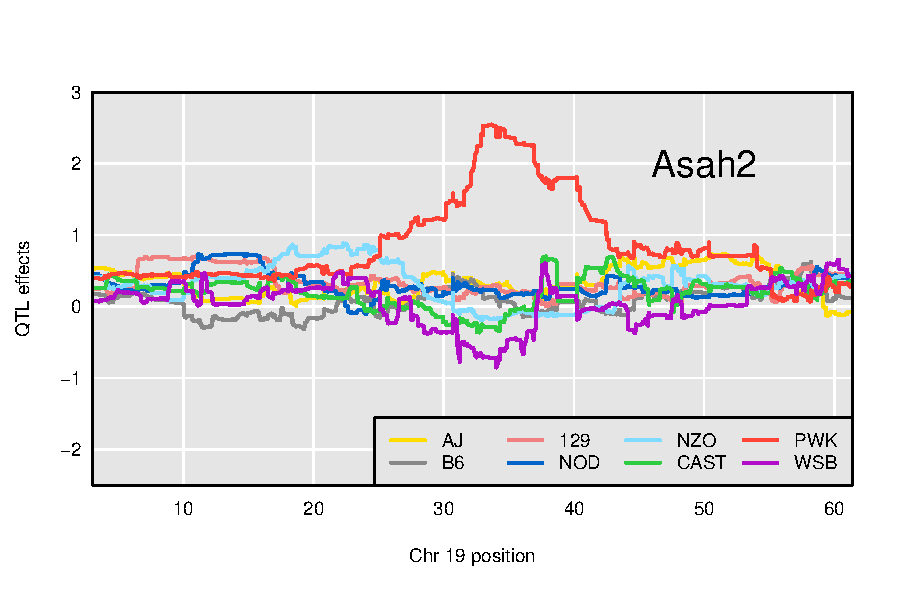
\includegraphics[width = \textwidth]{../Rmd/allele_effects_Asah2.pdf}
    \end{subfigure}%
    \begin{subfigure}[t]{0.5\textwidth}
        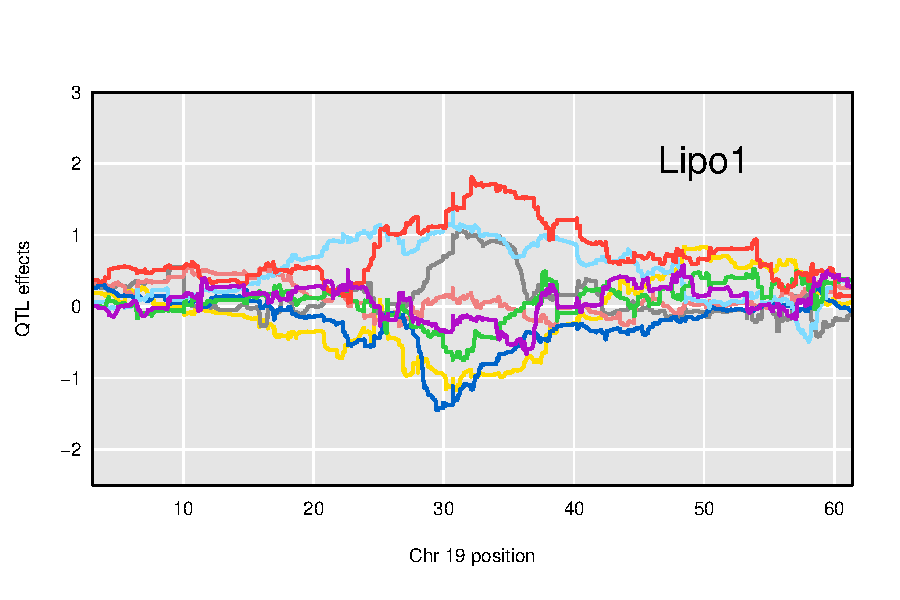
\includegraphics[width = \textwidth]{../Rmd/allele_effects_Lipo1.pdf}
    \end{subfigure}%
    
    \begin{subfigure}[t]{0.5\linewidth}
        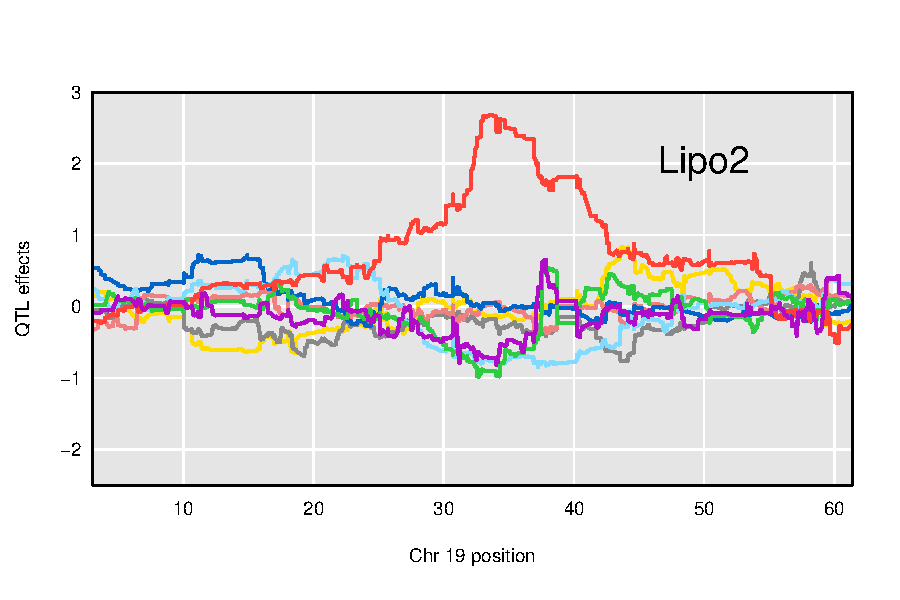
\includegraphics[width = \linewidth]{../Rmd/allele_effects_Lipo2.pdf}
    \end{subfigure}
    \begin{subfigure}[t]{0.5\linewidth}
        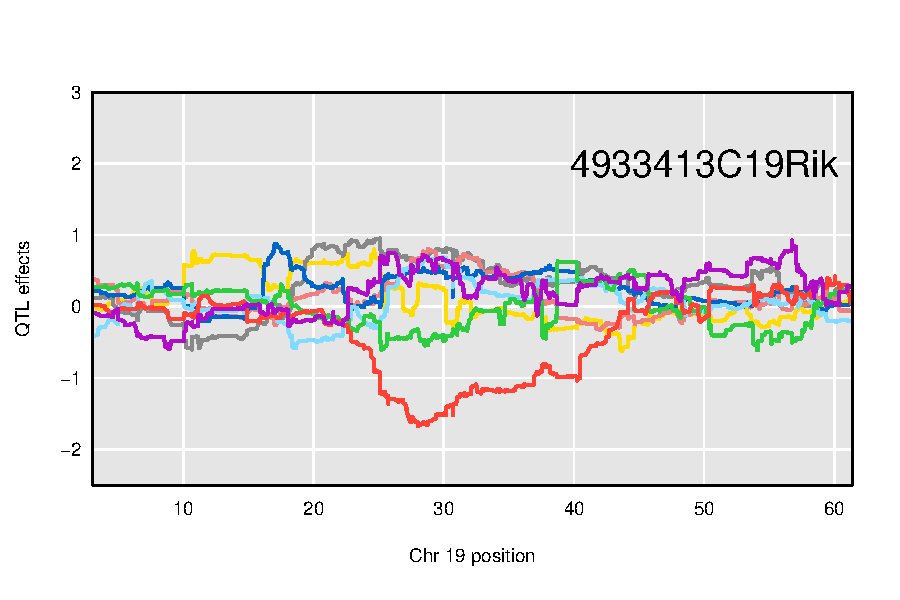
\includegraphics[width = \linewidth]{../Rmd/allele_effects_4933413C19Rik.pdf}
    \end{subfigure}
        \caption{Founder allele effects plots for Chromosome 19 for the four "anchor" gene expression traits reveal strong PWK effects (red line) for all four traits. For Asah2 (upper left panel), WSB has a strong negative effect, opposite the direction of the PWK effect.}\label{fig:founder-allele-effects}
\end{figure}




\subsection{Pleiotropy LRT vs. chromosomal position}

\begin{figure}
    \centering
    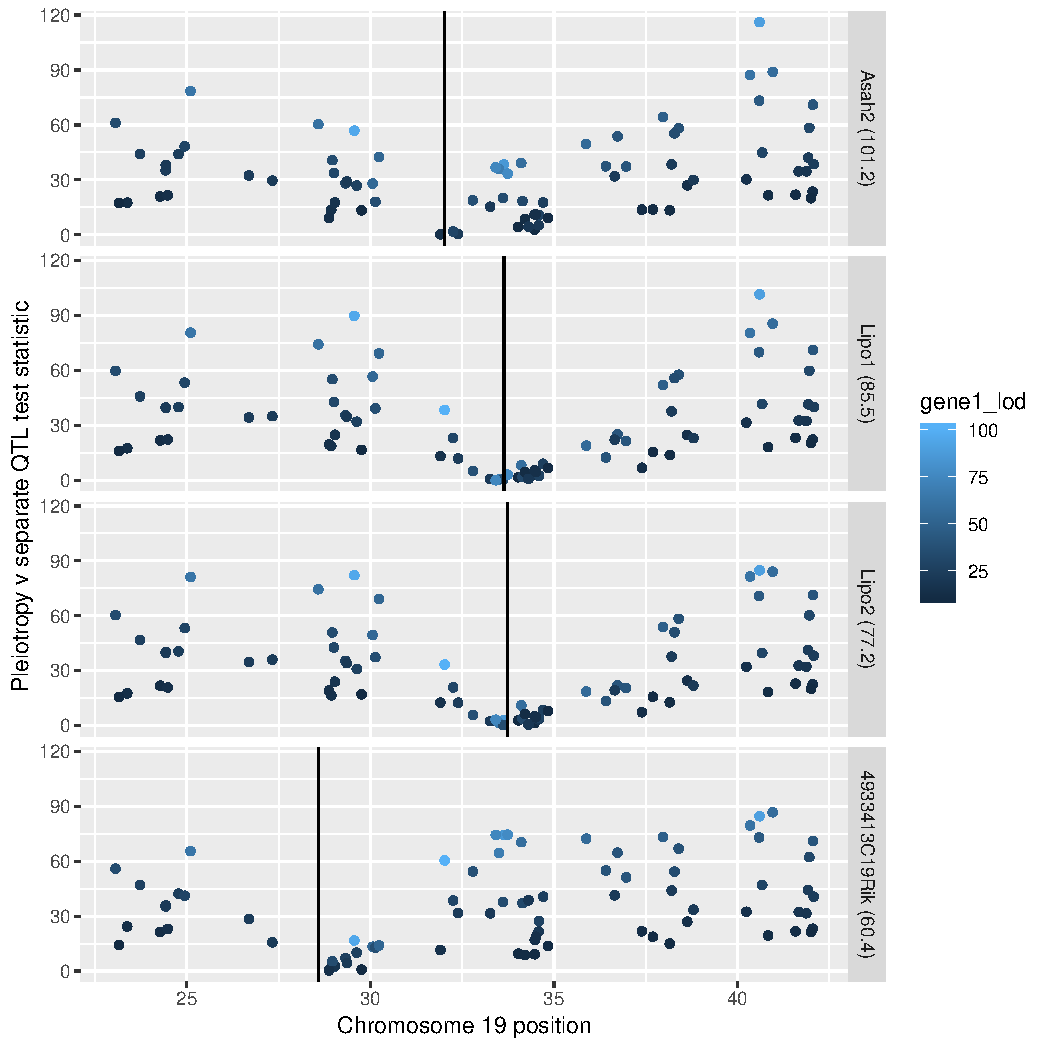
\includegraphics[width = \textwidth]{../Rmd/lrt-v-middle-of-gene.pdf}
    \caption{Caption}
    \label{fig:middle}
\end{figure}


\subsection{Pleiotropy likelihood ratio test statistics vs. univariate LOD peak heights}

\begin{figure}
    \centering
    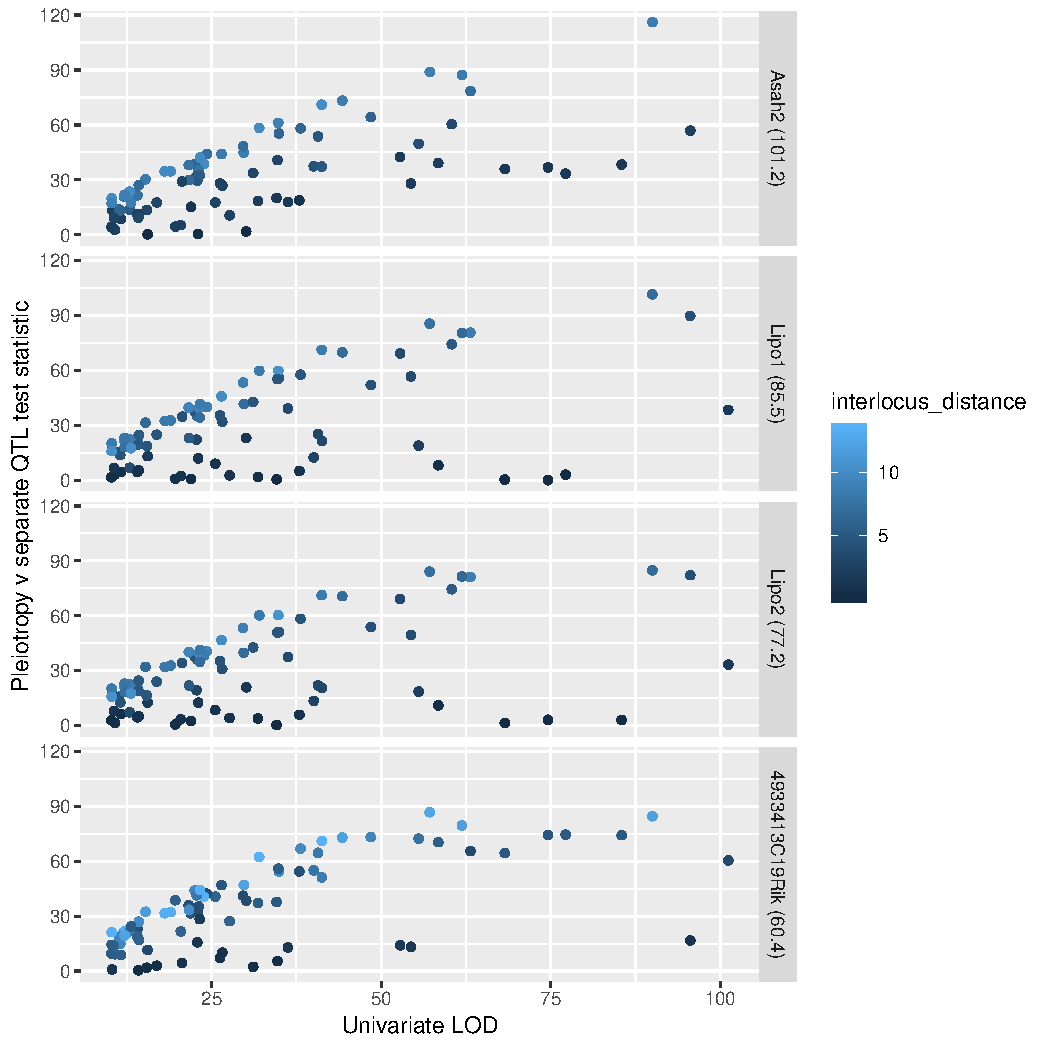
\includegraphics[width = \textwidth]{../Rmd/lrt-v-univariate-lod.pdf}
    \caption{Caption}
    \label{fig:lod}
\end{figure}


\subsection{Pleiotropy LRT vs. fitted values correlation}

\begin{figure}
    \centering
    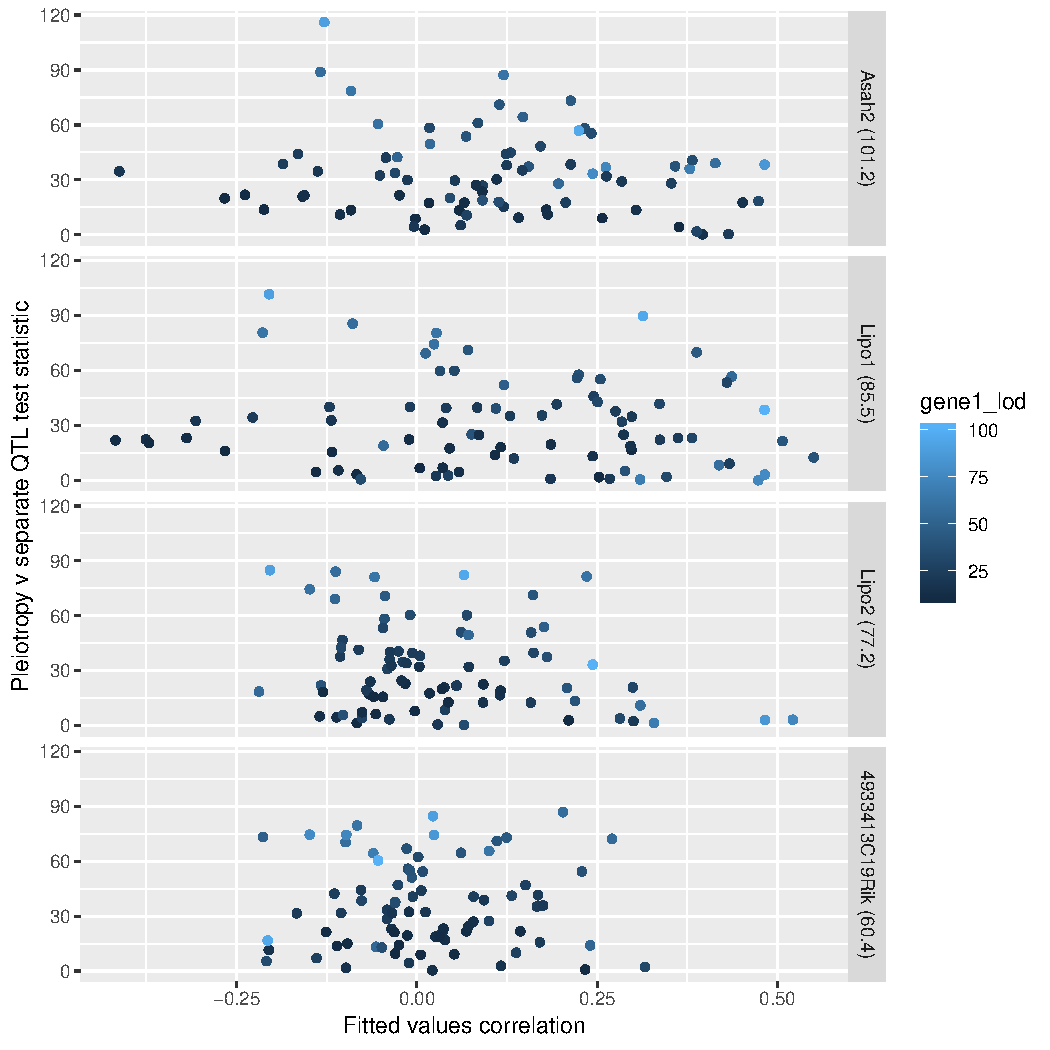
\includegraphics[width = \textwidth]{../Rmd/lrt-v-corr.pdf}
    \caption{Caption}
    \label{fig:cor}
\end{figure}

\section{Discussion}





\section{References}

\printbibliography
% latex table generated in R 3.5.2 by xtable 1.8-3 package
% Thu Jan  3 16:43:33 2019
\begin{table}[ht]
\centering
\begingroup\tiny
\begin{tabular}{lrrrr}
  \hline
symbol & start & end & peak\_position & lod \\ 
  \hline
C030046E11Rik & 29.52 & 29.61 & 29.55 & 95.58 \\ 
  Tctn3 & 40.60 & 40.61 & 40.59 & 90.00 \\ 
  Gm7237 & 33.41 & 33.42 & 33.67 & 74.61 \\ 
  Lipo4 & 33.50 & 33.52 & 34.00 & 68.23 \\ 
  Dock8 & 25.00 & 25.20 & 25.07 & 63.17 \\ 
  Sorbs1 & 40.30 & 40.40 & 40.48 & 61.89 \\ 
  Lipm & 34.10 & 34.12 & 34.06 & 58.43 \\ 
  Blnk & 40.93 & 40.99 & 40.76 & 57.16 \\ 
  A830019P07Rik & 35.84 & 35.92 & 35.60 & 55.54 \\ 
  Uhrf2 & 30.03 & 30.09 & 29.96 & 54.40 \\ 
  Mbl2 & 30.23 & 30.24 & 30.18 & 52.81 \\ 
  Myof & 37.90 & 38.04 & 38.05 & 48.46 \\ 
  Gm27042 & 40.59 & 40.59 & 40.61 & 44.27 \\ 
  Btaf1 & 36.93 & 37.01 & 36.90 & 41.25 \\ 
  Hoga1 & 42.05 & 42.07 & 42.09 & 41.23 \\ 
  Ppp1r3c & 36.73 & 36.74 & 36.53 & 40.69 \\ 
  Pcgf5 & 36.38 & 36.46 & 36.24 & 40.06 \\ 
  Slc35g1 & 38.40 & 38.41 & 38.35 & 38.11 \\ 
  Pten & 32.76 & 32.83 & 32.77 & 37.95 \\ 
  Gldc & 30.10 & 30.18 & 30.17 & 36.26 \\ 
  Lgi1 & 38.26 & 38.31 & 38.17 & 34.91 \\ 
  C330002G04Rik & 23.04 & 23.08 & 23.34 & 34.84 \\ 
  Ppapdc2 & 28.96 & 28.97 & 29.09 & 34.71 \\ 
  Gm8978 & 33.61 & 33.63 & 33.03 & 34.59 \\ 
  Mms19 & 41.94 & 41.98 & 41.98 & 32.03 \\ 
  Ankrd22 & 34.12 & 34.17 & 34.04 & 31.83 \\ 
  Cdc37l1 & 28.99 & 29.02 & 29.03 & 31.14 \\ 
  Sgms1 & 32.12 & 32.39 & 32.11 & 30.10 \\ 
  Entpd1 & 40.61 & 40.74 & 40.50 & 29.73 \\ 
  Cbwd1 & 24.92 & 24.96 & 24.73 & 29.65 \\ 
  Gm14446 & 34.59 & 34.60 & 34.28 & 27.65 \\ 
  Ermp1 & 29.61 & 29.65 & 29.70 & 26.57 \\ 
  Gm9938 & 23.72 & 23.73 & 23.87 & 26.46 \\ 
  Insl6 & 29.32 & 29.33 & 29.37 & 26.23 \\ 
  Slc16a12 & 34.67 & 34.75 & 34.71 & 25.54 \\ 
  Pgm5 & 24.68 & 24.86 & 25.00 & 24.30 \\ 
  Morn4 & 42.07 & 42.09 & 41.79 & 23.86 \\ 
  Exosc1 & 41.92 & 41.93 & 42.10 & 23.28 \\ 
  Smarca2 & 26.61 & 26.78 & 26.59 & 23.25 \\ 
  4930418C01Rik & 24.42 & 24.43 & 23.92 & 23.10 \\ 
  2700046G09Rik & 32.39 & 32.39 & 32.25 & 23.02 \\ 
  Kcnv2 & 27.32 & 27.34 & 27.14 & 22.88 \\ 
  1500017E21Rik & 36.61 & 36.71 & 37.07 & 22.78 \\ 
  Fra10ac1 & 38.19 & 38.22 & 38.35 & 22.48 \\ 
  Rnls & 33.14 & 33.39 & 34.17 & 21.94 \\ 
  Noc3l & 38.79 & 38.82 & 40.20 & 21.67 \\ 
  Pip5k1b & 24.29 & 24.56 & 24.15 & 21.62 \\ 
  Plgrkt & 29.35 & 29.37 & 29.37 & 20.65 \\ 
  Ifit3 & 34.58 & 34.59 & 34.28 & 20.45 \\ 
  Fas & 34.29 & 34.33 & 34.20 & 19.65 \\ 
  Slit1 & 41.60 & 41.74 & 41.70 & 18.95 \\ 
  Rrp12 & 41.86 & 41.90 & 41.71 & 18.09 \\ 
  Ak3 & 29.02 & 29.05 & 29.55 & 16.90 \\ 
  A1cf & 31.87 & 31.95 & 32.11 & 15.56 \\ 
  4430402I18Rik & 28.90 & 28.97 & 29.37 & 15.43 \\ 
  Pdlim1 & 40.22 & 40.27 & 40.25 & 15.25 \\ 
  Gm26902 & 34.47 & 34.48 & 36.15 & 14.26 \\ 
  Plce1 & 38.48 & 38.79 & 38.42 & 14.26 \\ 
  Slc1a1 & 28.84 & 28.91 & 28.97 & 14.18 \\ 
  Fam122a & 24.48 & 24.48 & 24.08 & 14.07 \\ 
  Lipa & 34.49 & 34.53 & 34.29 & 14.06 \\ 
  Mamdc2 & 23.30 & 23.45 & 23.35 & 13.12 \\ 
  Kif11 & 37.38 & 37.42 & 37.33 & 12.93 \\ 
  4933411K16Rik & 42.05 & 42.05 & 42.08 & 12.92 \\ 
  Ccnj & 40.83 & 40.85 & 40.59 & 12.19 \\ 
  Gm340 & 41.58 & 41.59 & 41.30 & 12.17 \\ 
  Fxn & 24.26 & 24.28 & 24.31 & 12.07 \\ 
  Stambpl1 & 34.19 & 34.24 & 34.28 & 11.62 \\ 
  Pde6c & 38.13 & 38.18 & 38.07 & 11.54 \\ 
  Cyp26a1 & 37.70 & 37.70 & 37.48 & 11.35 \\ 
  Ch25h & 34.47 & 34.48 & 32.50 & 10.74 \\ 
  Pank1 & 34.81 & 34.88 & 35.55 & 10.61 \\ 
  9930021J03Rik & 29.71 & 29.81 & 28.71 & 10.32 \\ 
  Klf9 & 23.14 & 23.17 & 23.34 & 10.26 \\ 
  Ubtd1 & 41.98 & 42.03 & 41.71 & 10.25 \\ 
  Lipk & 34.01 & 34.05 & 34.29 & 10.23 \\ 
   \hline 
\end{tabular}
\endgroup
\caption{Annotations for 76 non-anchor genes on Chromosome 19.}
\end{table}

\end{document}
